\label {unit4}

% View Menu

\section{View Menu}

The \textsf{View} menu provides several useful options for coding and
looking at large amounts of data.

\begin{itemize}
\item[Zoom] To change the amount of data seen in the MultiSeq window,
you can zoom in and out.  As you zoom farther out (choosing a percentage
that is smaller) MultiSeq will makes the sequence letters smaller and
smaller until you will only see the background colors and then, not even
that.  If you need to see the entire sequence, the \textsf{Zoom Window},
discussed below, might be more useful.
\item [Coloring]
You can choose to color the sequences by a wide range of attributes.
First, you can choose \emph{what} you want to color by choosing
\textsf{Apply to All}, \textsf{Group}, or \textsf{Marked}.  Then, you
can choose the coloring method that you wish to apply.  

For \textsf{Qres}, traditionally, Q has meant ``the fraction of
     similar native contacts'' between the aligned residues in two
     proteins\footnote {Eastwood, M.P., C. Hardin, Z. Luthey-Schulten,
     and P.G. Wolynes. ``Evaluating protein structure-prediction schemes
     using energy landscape theory.''  IBM J . Res. Dev. 45: 475-497.
     2001}, or in two different conformational states of the same
     protein.  When Q = 1, it indicates that the structures are
     identical.  When Q has a low score (\textit{0.1}), it means the
     structures do not align well, or, in other words, only a small
     fraction of the C-alpha atoms superimpose.  You will discover that
     homologs typically have Q$\ge$0.4.  Q per residue is the
     contribution from each residue to the overall average Q score.  For
     more information see Appendix A.

For \textsf{Sequence Identity}, the aligned domains are colored by how
much of the sequence is conserved. The \textsf{Sequence Identity}
coloring method colors each amino acid according to the degree of
conservation within the alignment: blue means highly conserved, wheras
red means very low or no conservation.

\item[Highlight Style]
\textsf{Highlight Style} is an option for the OpenGL diplay.  The style
refers to drawing method in VMD\footnote {For more information about
drawing methods, please refer to the VMD manual.}.  This option allows a
user to highlight residues of a structure in the sequence display and
see the areas simultaneously highlighted in the OpenGL display.

\item[Highlight Color]
\textsf{Highlight Color} is another option for the OpenGL diplay.
Alongside \textsf{Highlight Style}, \textsf{Highlight Color} is the
color or coloring method\footnote{For more information, please refer to
the VMD manual} used in the OpenGL display when highlighting residues in
the Sequence Display.  The default \textsf{Highlight Color} is yellow.

\item[Color Scale]  Once you have chosen a coloring, you might wonder
what the specific colors mean.  The \textsf{Color Scale} option will
show you the scale of colors according to value.

\begin{figure}[here]
 \centerline{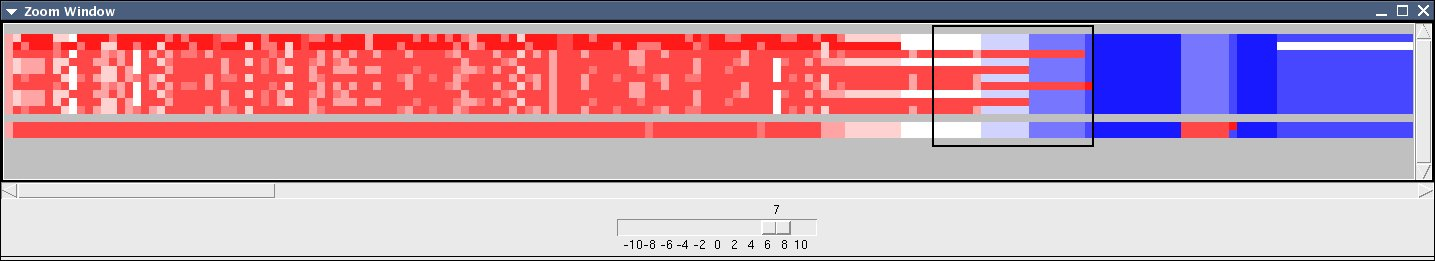
\includegraphics [width=5in]{./pictures/zoomWindow.jpg}}
 \caption{Zoom Window}
\label{fig:zoomWindow}
\end{figure}
\item [Zoom Window] (See Fig.~\ref{fig:zoomWindow}) If you need to see
the entire collection of sequences and quickly move from area to area,
the \textsf{Zoom Window} will be useful to you.  It shows the entire
sequence palette.  You can choose the zoom factor using the sliding bar
at the bottom of the window, and the black box shows you the area of the
sequences that are currently visible in the MultiSeq window.  To see
other areas, just click the mouse and the black box will be moved to the
mouse pointer location.

Note:  When you have the \textsf{Zoom Window} open, the MultiSeq window
will redraw more slowly.  If this is a problem for you, just close the
\textsf{Zoom Window} and reopen as needed.

\end{itemize}

